% GENERATED BY sshrc_figures.py - edit that file, not this one.
% The document that inputs this file supplies the float, the caption and the label.
% Stream B. Committees, left to right within each year: Philosophy, History, Fine arts, Literature, Medieval, classics and religious studies, Sociology, Geography, Psychology (10A, 10B), Political science, Education (12A, 12B, 12C), Anthropology, Linguistics, Communications, Law and criminology.
\definecolor{sshrcA}{HTML}{2A78D6}
\definecolor{sshrcB}{HTML}{EB6834}
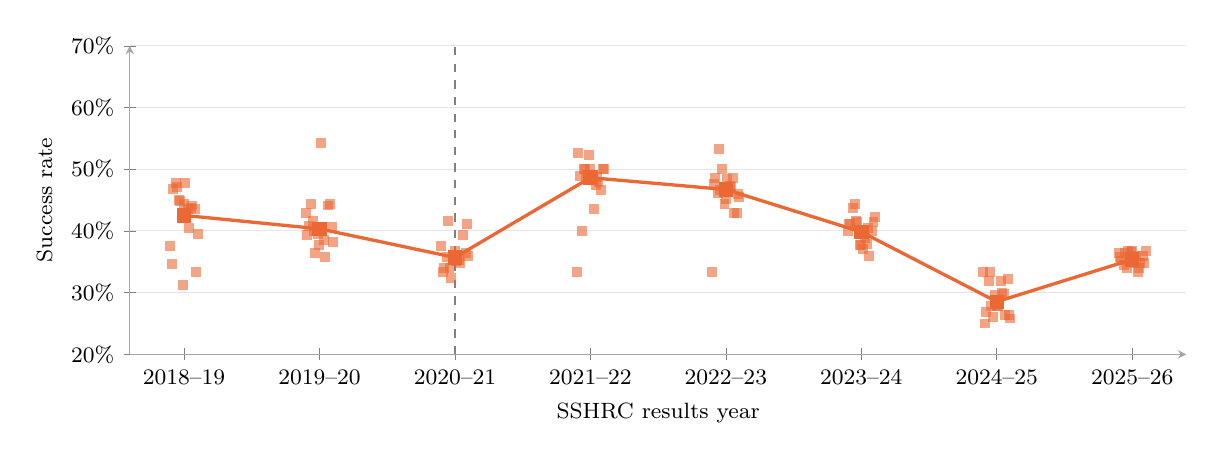
\begin{tikzpicture}
\begin{axis}[
  width=15cm, height=5.5cm,
  xmin=2017.6, xmax=2025.4, ymin=20, ymax=70,
  xtick={2018,2019,2020,2021,2022,2023,2024,2025}, xticklabels={2018--19,2019--20,2020--21,2021--22,2022--23,2023--24,2024--25,2025--26},
  axis x line=bottom, axis y line=left, axis line style={gray!70},
  ymajorgrids, grid style={gray!20},
  tick label style={font=\footnotesize}, label style={font=\footnotesize},
  xlabel={SSHRC results year}, ylabel={Success rate}, ylabel style={align=center},
  clip=false,
  ytick distance=10, yticklabel={\pgfmathprintnumber{\tick}\%},
]
\draw[gray, dashed, line width=0.7pt] (axis cs:2020,20) -- (axis cs:2020,70);
\addplot[only marks, mark=square*, mark size=1.8pt, color=sshrcB,
  mark options={fill opacity=0.6, draw opacity=0}]
  coordinates {(2018.06,44.12) (2018.09,33.33) (2018.03,43.48) (2018.04,40.54) (2018.05,43.75) (2017.92,46.81) (2017.97,44.90) (2017.91,34.62) (2018.10,39.47) (2018.08,43.48) (2017.94,47.83) (2017.95,47.06) (2017.90,37.50) (2018.01,47.73) (2017.99,31.25) (2018.00,44.44) (2017.96,45.00) (2019.06,44.12) (2019.09,40.62) (2019.03,38.46) (2019.04,35.71) (2018.92,40.82) (2018.97,36.36) (2018.91,39.39) (2019.10,38.24) (2019.08,44.44) (2018.94,44.44) (2018.95,41.67) (2018.90,42.86) (2019.01,54.29) (2018.99,39.53) (2019.00,37.78) (2018.96,40.00) (2019.90,37.50) (2019.91,33.33) (2019.92,34.04) (2019.94,35.71) (2019.95,41.67) (2019.96,34.00) (2019.97,32.43) (2019.99,35.42) (2020.00,36.73) (2020.01,35.19) (2020.03,35.29) (2020.04,34.85) (2020.06,39.39) (2020.08,36.36) (2020.09,41.18) (2020.10,35.90) (2020.90,33.33) (2020.91,52.63) (2020.92,48.89) (2020.94,40.00) (2020.95,50.00) (2020.96,50.00) (2020.97,48.65) (2020.99,52.38) (2021.00,50.00) (2021.01,48.78) (2021.03,43.59) (2021.04,47.50) (2021.05,48.78) (2021.06,48.00) (2021.08,46.67) (2021.09,50.00) (2021.10,50.00) (2021.90,33.33) (2021.91,47.62) (2021.92,48.57) (2021.94,46.15) (2021.95,53.33) (2021.96,46.67) (2021.97,50.00) (2021.99,44.44) (2022.00,45.24) (2022.01,48.39) (2022.03,47.22) (2022.04,47.06) (2022.05,48.57) (2022.06,42.86) (2022.08,42.86) (2022.09,45.95) (2022.10,45.45) (2022.90,40.00) (2022.91,41.18) (2022.92,41.18) (2022.94,43.75) (2022.95,44.44) (2022.96,41.67) (2022.97,41.46) (2022.99,37.78) (2023.00,37.78) (2023.01,37.14) (2023.03,38.89) (2023.04,37.84) (2023.05,40.54) (2023.06,36.00) (2023.08,40.00) (2023.09,41.38) (2023.10,42.31) (2023.90,33.33) (2023.91,25.00) (2023.92,26.92) (2023.94,31.82) (2023.95,33.33) (2023.96,27.91) (2023.97,26.00) (2023.99,29.63) (2024.00,27.87) (2024.01,27.87) (2024.03,31.91) (2024.04,30.00) (2024.05,29.79) (2024.06,26.32) (2024.08,32.14) (2024.09,26.42) (2024.10,25.81) (2024.90,36.36) (2024.91,35.71) (2024.92,35.21) (2024.94,34.48) (2024.95,36.36) (2024.96,34.00) (2024.97,36.67) (2024.99,36.62) (2025.00,36.76) (2025.01,34.72) (2025.03,36.00) (2025.04,33.33) (2025.05,34.00) (2025.06,34.88) (2025.08,36.00) (2025.09,34.78) (2025.10,36.67)};
\addplot[color=sshrcB, line width=1.2pt, mark=square*, mark size=2pt] coordinates {(2018.00,42.52) (2019.00,40.34) (2020.00,35.70) (2021.00,48.63) (2022.00,46.71) (2023.00,39.84) (2024.00,28.53) (2025.00,35.38)};
\end{axis}
\end{tikzpicture}
